\section{Data and Methodology}\label{Data}\thispagestyle{SectionFirstPage} % Hide headers on the first page of the section
\subsection{Research Design}
We are interested in assessing how Twitter network structures differ among distinct topics of discussion. We explore the differences between such topic-network structures in terms of their network topology measures and how these affect the number of interactions between pairs of users. For this purpose, we first need to collect the data and retrieve tweets conversations based on selected topics. Next, we perform a regression analysis on these networks, where the predictors are the nodes' respective network measures, and the explained variable is the number of interactions between every pair of nodes in the network.
Before explaining our methodology in more detail, we set out some basic definitions of fundamental concepts of graph theory and social network analysis.

A social network is a network (or graph) of \textit{interactions} or \textit{relationships} between actors \citep{aggarwal:2011}. The actors are called \textit{nodes}, whereas their interactions are called \textit{edges}, links, or ties. Social networks are not restricted to a purely online form. In fact, they have been studied by sociologists for generations before the advent of OSN \citep[see, e.g.,][]{milgram:1967}. However, in the context of OSN, users are often the nodes who form ties or connections (edges) among themselves to exchange content like text, images, videos, or in another form. In this paper, the nodes represent the interacting users and the edges their tweets, retweets, mentions, or replies.

\begin{figure}[ht]
\centering{}\caption{Nodes and edges in undirected and directed graphs.\label{fig:directed-undirected}}
\begin{center}
\begin{tikzpicture}[scale=1.5]
    \node[shape=circle, draw=black, minimum size=0.9cm] (i) at (1,2) {$i$};
    \node[shape=circle, draw=black, minimum size=0.9cm] (j) at (0,0) {$j$};
    \node[shape=circle, draw=black, minimum size=0.9cm] (k) at (2,0) {$k$};

    \path [-](i) edge node[left=4pt] {$e_{i,j} = e_{j,i}$} (j);
    \path [-](j) edge node[below=4pt] {$e_{j,k} = e_{j,k}$} (k);
    \path [-](k) edge node[right=4pt] {$e_{k,i} = e_{i,k}$} (i);

    \node[shape=circle, draw=black, minimum size=0.9cm] (i) at (5,2) {$i$};
    \node[shape=circle, draw=black, minimum size=0.9cm] (j) at (4,0) {$j$};
    \node[shape=circle, draw=black, minimum size=0.9cm] (k) at (6,0) {$k$};

    \path [->,>=triangle 45](i) edge node[left=4pt] {$e_{i,j}$} (j);
    \path [->,>=triangle 45](j) edge node[below=4pt] {$e_{j,k}$} (k);
    \path [->,>=triangle 45](k) edge node[right=4pt] {$e_{k,i}$} (i);

    \node[shape=circle, draw=none] (label1) at (1,-1) {Undirected graph};
    \node[shape=circle, draw=none] (label2) at (5,-1) {Directed graph};
\end{tikzpicture}
\end{center}
\vspace{-60pt}
\end{figure}

A network can be \textit{directed}, like follow relationships on Twitter, or \textit{undirected}, like mutual friendships on Facebook (see Figure \vref{fig:directed-undirected}). In directed graphs, asymmetric binary relations may occur, hence the edge from node $i$ to node $j$ is different than the one from $j$ to $i$. Moreover, a network may be \textit{weighted}, where a weight is set for each edge or, whenever multiple edges can occur between two nodes (e.g., in a conversation of tweets), the weight can be the number of edges between these nodes.
In our case, in a weighted graph $\mathcal{G}$, let $e_{i,j}$ be the edge between node $i$ and node $j$, and let $w_{i,j}$ be the weight on edge $e_{i,j}$ computed as the number of interactions between $i$ and $j$. The total weight $w_i$ of the node $i$ can be thus defined as the sum of weights of all its edges, that is $w_i = \sum_{k=1}^{d_i} w_{i,k}$, where $d_i$ denotes its degree. The \textit{degree} of a node is defined as the number of edges for that given node – i.e., how many connections a node has in the network. The weighted degree is similarly based on the number of edges for that node, but ponderated by the weight of such edges – i.e., the number of interactions between a pair of nodes.
One final notable network concept is related to \textit{density}, which stands for the proportion of edges present in a network compared to the number of all potentially possible edges - i.e., the completeness of a network. Density is therefore defined as
${Network\, Density = \frac{No.\, of\, actual\, edges}{No.\, of\, potential\, edges} = \frac{No.\, of\, actual\, edges}{\frac{N\; (N-1)}{2}}}$,
where $N$ is the total number of nodes in the network.

To perform our study, we require nodes and edges tables for each topic of discussion. The former are tables with data for each node, while the latter contain information on the edges between each pair of nodes. In our case, nodes tables include network topology measures for each node, while edges tables specify which are the source and target nodes, and the weight of their edge. We provide examples of the structure of these tables in Appendix \vrefrange{nodestable}{metricstable}.

The process to obtain the final data set for each topic consists of four main sequential stages.
First, primary data is collected in real-time via the Twitter API endpoints, then stored on a MongoDB (NoSQL) database for real-time querying and visualization, as well as on an Amazon Web Services (AWS) S3 bucket for long-term storage.
Secondly, data is cleaned, selected, and prepared with a five-step pipeline in Python. These scripts transform the raw data set into nodes and edges tables for each analyzed topic.
Subsequently, the latter tables are imported to Gephi in order to visualize their graph structures and compute network measurements.
Lastly, we import into an R program the updated tables with new measures exported from Gephi. This R script constructs adjacency lists and runs three generalized linear models for each topic, where the covariates are node-level network metrics. First, we run a multiple regression model on the number of interactions for every pair of users. Secondly, a logistic model to assess the probability of interaction between two users. Finally, a conditional (filtered) multiple regression model on the number of interactions, only for those pairs of users that interacted with each other.

In this chapter, we further illustrate the rationale behind each step in the pipeline. To enable reproducibility of our research, we publish all our scripts on GitHub with open access\footnote{The repository can be accessed from: \url{https://github.com/andreantonacci}.}.
% Too short
\subsection{Data Collection}
\subsubsection{Twitter Real-time Filter API}
We conduct all the analyses in this paper on primary data collected via the Twitter real-time filter API\footnote{\url{https://developer.twitter.com/en/docs/tweets/filter-realtime/overview}.} (standard plan) – or streaming API. We commence the collection of data on May 16, 2019, at 12:50:00 UTC, using the \texttt{tweepy}\footnote{\url{https://www.tweepy.org}.} library for Python to access the Twitter API.

The API returns public tweets that match one or more filters (e.g., a keyword, hashtag, username, or location) in a JSON response format\footnote{A full list of JSON tweet objects and a tweet data dictionary can be found here: \url{https://developer.twitter.com/en/docs/tweets/data-dictionary/overview/tweet-object}.}. The latency from the tweet publication to its delivery on the API is typically within seconds. The default access level (standard plan) to the Twitter API is free but subject to some limitations: it allows for tracking up to 400 keywords and returns at most 1\% of all tweets being published on Twitter at a given moment \citep{morstatter:2014}. Because of the limited resources available for this project, we cannot set up an enterprise plan and utilize the PowerTrack API\footnote{\url{https://developer.twitter.com/en/docs/tweets/filter-realtime/overview/powertrack-api}.}, which provides full-fidelity data and reliable connectivity instead. However, researchers have shown that the resulting data sets from the streaming API are a representative sample and truthfully reflect the activity patterns of Twitter users \citep{morstatter:2013, morstatter:2014, wang:2015}.

To overcome the limitation of 400 keywords and ensure a continuous flow of tweets, we run our script on two Amazon Elastic Compute Cloud (Amazon EC2) instances\footnote{The instance type is \texttt{m5.xlarge}, powered by Intel Xeon Platinum 8175 processors, 4 vCPU, and 16GB of memory.}. Each instance executes the same script 24 hours a day but tracks a different set of keywords and connects to the API with a different Twitter developer account – i.e., with a different API key and access token. In this way, we can track up to 800 keywords but run the risk of collecting the same tweet twice – i.e., in the case that a tweet contains two or more hashtags, each one tracked on a different EC2 instance, both of the machines may collect it. We address this issue a posteriori, as illustrated in section \vref{electionstats}.

A second limitation of this approach is that the data set may contain only a portion of a conversation, which happens if the initial tweet (called \textit{seed} or conversation starter) is not part of the collection returned by the API. In such a case, we treat the earliest tweet available in the conversation tree (a tweet replying to another one that is not part of our data set) as the initial tweet.

The collection process stopped on June 2, 2019, with a total of 21,337,037 unique tweets. We tracked approximately 800 different keywords, which include:
\begin{itemize}
\item General hashtags on the elections (in all the different languages spoken in the EU): e.g., \#EUElections, \#EUvaalit2019, \#EP2019;
\item All the European Parliament groups' handles and official hashtags: e.g., @ALDE, \#ALDE, @EPP, \#EPP;
\item All the major national parties' handles (i.e., those which have at least a seat in the national parliament): e.g., @groen, @PdA\_Austria, @LegaSalvini;
\item All the national party's leaders' handles: e.g., @theresa\_may, @luigidimaio, @pablocasado\_;
\item Keywords on popular politics-related topics and challenges faced by the EU at that time (in all the different languages spoken in the EU): \texttt{brexit}, \texttt{eu institutions}, \texttt{fake news}, \texttt{gender equality}, \texttt{lgbt rights}, \texttt{populism}, \texttt{public debt}, \texttt{refugees}, \texttt{single market}, \texttt{terrorism}, \texttt{unemployment}.
\end{itemize}
A complete list of tracked keywords and a logbook of events that occurred during the collection process can be found in Appendix \vref{appendix-b}.
\subsubsection{Electionstats: MongoDB and Real-time Visualization}\label{electionstats}
Electionstats\footnote{The dashboard can be accessed from: \url{https://electionstats.eu}.} is a side project of this research study. It consists of a visualization dashboard of insights retrieved from the collected tweets during the electoral period that updates in real-time. Because the objective of this side project is outside the scope of the present study, we do not deepen into its characteristics\footnote{However, we make the scripts available in the project’s repository.}. Nonetheless, it is necessary to outline how Electionstats affects our data collection and storage strategy.

Storing data to a secure cloud service seems the most efficient solution if there is not the need for live data querying. Instead, in this case, we first add an intermediate step: we import our data to a NoSQL database (MongoDB\footnote{The cluster tier is M30, with 7.5GB of RAM, 101GB of storage, encrypted, with MongoDB 4.0 and hosted on the Google Cloud Platform.}), which allows us to run the (almost) real-time\footnote{Or rather, frequent ones.} queries needed for the live dashboard. To do so, we write the raw data returned from the API to a new JSON file every five minutes. Another Python script then scans the directory where the files are saved, parses the tweets, and imports them to MongoDB only if their file is older than five minutes and their tweet ID does not exist in the database already. Lastly, it also uploads the raw files to an Amazon Simple Storage Service (Amazon S3) bucket and removes the file locally, if the upload is successful.
\subsubsection{Long-term Storage on Amazon S3}\label{s3}
Once the official electoral results are published, and our collection is complete, there is no need for further updates of the Electionstats dashboard, and thus for a MongoDB database. We export all data from the database to three equally sized JSON files\footnote{For simplicity, we refer to them in tables and figures as, respectively, \texttt{eu2019}, \texttt{eu2019v2}, and \texttt{eu2019v3}.} and upload them to an encrypted Amazon S3 bucket for long-term storage. We conduct all analyses in this study on derived data from a merged file (master data file) that is the sum of these three.
\subsection{Data Hygiene and Preparation in Python}
We perform our data selection, modeling, and analysis on a single server with Windows Server 2012 R2 Standard, two Intel Xeon Gold 6126 CPU at 2.60GHz, and 512GB of RAM available. Because the resources needed for a computer cluster architecture are too expensive for this project, we must first reduce our data to enable further wrangling and analysis.

The algorithm employed to sample tweets from the master data file retains one line out of ten lines. This sampling method ensures that the resulting data set is still a representative sample, because the tweets in the master data file are ordered by timestamp, and the retained ones encompass the entire electoral period. The final sampled data set is a tenth of the size of the original master data file (16.22GB), with 2,259,717 unique tweets.

Subsequently, we employ a five-step pipeline to prepare our data and obtain nodes and edges tables for each topic. The overall process is run in Python 3 and illustrated in the flowchart (see Figure \vref{fig:pipeline-flowchart}).
% Python Pipeline
\begin{figure}
  \centering{}\caption{Data wrangling pipeline in Python.\label{fig:pipeline-flowchart}}
  \begin{center}
  \scalebox{0.8}{\begin{tikzpicture}[node distance=1cm, scale=0.75, every node/.style={transform shape}]
  \node (start) [startstop] {Start};
  \node (in) [io, below=of start] {Master file + topic files};
  \node (pro1) [process, below=of in] {Get Conversation IDs};
  \node (for) [chamfered rectangle, chamfered rectangle xsep=2cm, draw, text centered, text width=2cm, minimum width=2cm]  [below=of pro1] {For topic in topics};
  \node (pro2) [process, below=of for] {Filter Conversations};
  \node (pro3) [process, below=of pro2] {Parse};
  \node (pro4) [process, below=of pro3] {Get Nodes};
  \node (pro5) [process, below=of pro4] {Get Edges};
  \node (out) [io, below=of pro5] {Nodes and Edges tables};
  \node (stop) [startstop, below=of out] {End};

  \draw [arrow] (start) -- (in);
  \draw [arrow] (in) -- (pro1);
  \draw [arrow] (pro1) -- (for);
  \draw [arrow] (for) -- node[right=4pt] {T} (pro2);
  \draw [arrow] (pro2) -- (pro3);
  \draw [arrow] (pro3) -- (pro4);
  \draw [arrow] (pro4) -- (pro5);
  \draw [arrow] (pro5) -- (out);
  \draw [arrow] (out.east) -- ++ (2.5 cm,0) |- (for.east);
  \draw [arrow] (for.west) -- ++ (-2.5 cm,0) node[above=4pt, xshift=1.25cm] {F} |- (stop.west);
  \end{tikzpicture}}
  \end{center}
\end{figure}
The first algorithm creates a list of unique tweets – identified by their ID – that are part of a conversation (see Algorithm \vref{getConversationId} with the pseudocode). We define such tweets as those that either started a conversation (seeds) – i.e., tweets that have been retweeted or replied to by another user at least once – or extended one by retweeting, quoting, or replying previous users in the sequence. This task is remarkably easy because we do not need to reconstruct the entire conversation tree. We simply filter all the tweets that are either a retweet, a quote, or a reply. Then, we store both their tweet ID and the ID of the tweet they are interacting with. In this way, we are sure to retain the seed IDs too because they must emerge from their retweets, quotes, and replies.
% Algorithm 1
\begin{algorithm}[ht]
  \caption{Get Conversation IDs}\label{getConversationId}
  \begin{algorithmic}[1]
  \State \textbf{Input:} $master\;file$
  \State \textbf{Output:} $conversation\;ids\;file$
  \State Initialize $toBeExported$ as empty array
  \State \textbf{read} $allTweets$ \textbf{from} $master\;file$
  \For {$tweet$ \textbf{in} $allTweets$}
    \If {$tweet$ \textbf{is not} valid}\Comment{skip empty lines}
      \State skip
    \EndIf
    \If {$tweet$ \textbf{is a} retweet \textbf{or is a} quote \textbf{or is a} reply}
      \State $toBeExported\gets tweet.id$
      \If {$tweet$ \textbf{is} a retweet}
        \State $toBeExported\gets tweet.seedId$
      \EndIf
      \If {$tweet$ \textbf{is} a quote}
        \State $toBeExported\gets tweet.seedId$
      \EndIf
      \If {$tweet$ \textbf{is} a reply}
        \State $toBeExported\gets tweet.seedId$
      \EndIf
    \EndIf
  \EndFor
  \State save $toBeExported$ to $conversation\;ids\;file$
  \end{algorithmic}
\end{algorithm}

All topics share this first step of the pipeline, and its script is invoked only once. The subsequent algorithms are executed for each topic instead. The computational complexity of our analysis in R (see section \vref{Models}) sets a limit upon the number of topics we can analyze. Hence, we select those we deem the most relevant and equally widespread in all the Member States. Because of the different relative importance in the public opinion of different States, we exclude the following topics from further analysis: \texttt{eu institutions}, \texttt{lgbt rights}, \texttt{public debt}. We also dismiss \texttt{gender equality} and \texttt{single market} because too few tweets appear in our sample – only 17 and 6 nodes, respectively – and \texttt{ep2019} because it does not identify a discussion topic. Instead, it refers to an event whose discussions do not revolve around a single topic. Finally, we exclude \texttt{fake news} due to technical difficulties. As a consequence, we perform our analysis on the following five discussion topics: \texttt{brexit}\footnote{We further sample \texttt{brexit} nodes (but not their respective edges and target nodes) because of the large volume of tweets collected. The final data set contains 4,843 nodes and 9,226 edges.}, \texttt{populism}, \texttt{refugees}, \texttt{terrorism}, and \texttt{unemployment}.
Appendix \vref{topic-file} provides an example of a topic file, which is a list of the tracked keywords for that specific topic.

The second algorithm selects only contributing users to a specified conversation filtered by topic (see Algorithm \vref{filterConversation}).  In order to further progress through the pipeline, a tweet must thus satisfy two conditions. Its tweet ID must be in the list of IDs that take part in a conversation, and at least one of its hashtags must be in the list of tracked keywords for a given topic note. More precisely, a perfect match between the hashtag and the tracked keyword is not required, because the tracked keyword can also be part of the hashtag. For instance, a tweet with the hashtag \texttt{\#IranianRefugeesInTurkey} can also satisfy this condition because it contains the tracked string \texttt{refugees}. As the outcome of this script, we obtain a filtered JSON file for each topic, which still contains full information for the selected tweets.
% \begin{multicols}{2}
% Algorithm 2
\begin{algorithm}
  \caption{Filter Conversations}\label{filterConversation}
  \begin{algorithmic}[1]
  \State \textbf{Input:} $master\;file$, $conversation\;ids\;file$, $current\;topic\;file$
  \State \textbf{Output:} $filtered\;tweets\;file$
  \State initialize $toBeExported$ as empty array
  \State \textbf{read} $conversationIds$ \textbf{from} $conversation\;ids\;file$\Comment{all tweets part of a conversation}
  \State \textbf{read} $topics$ \textbf{from} $current\;topic\;file$
  \State \textbf{read} $allTweets$ \textbf{from} $master\;file$
  \For {$tweet$ \textbf{in} $allTweets$}
    \If {$tweet$ \textbf{is not} valid}
      \State skip
    \EndIf
    \State Initialize $hashtagsList$ as empty array
    \If {len($tweet.hashtags$) $> 0$}\Comment{look for hashtags only if present}
      \For {$hashtag$ \textbf{in} $tweet.hashtags$}
        \State $hashtagsList\gets hashtag$
      \EndFor
    \EndIf
    \If {$tweet.id$ \textbf{in} $conversationIds$}\Comment{retain only matching tweets}
      \For {$hashtag$ \textbf{in} $hashtagsList$}
        \For {$topic$ \textbf{in} $topics$}
          \If {$topic$ \textbf{in} $hashtag$}
            \State $toBeExported\gets tweet$
          \EndIf
        \EndFor
      \EndFor
    \EndIf
  \EndFor
  \State save $toBeExported$ to $filtered\;tweets\;file$
  \end{algorithmic}
\end{algorithm}
% \end{multicols}

In the third step, we parse each JSON file to maintain only relevant fields and further reduce the file size. We retain selected fields, as shown in Algorithm \vref{parse}, and write the data on a CSV file for each topic.
% Algorithm 3
\begin{algorithm}
  \caption{Parse JSON file and convert to CSV}\label{parse}
  \begin{algorithmic}[1]
  \State \textbf{Input:} $filtered\;tweets\;file$
  \State \textbf{Output:} $parsed\;tweets\;file$
  \State \textbf{read} $filteredTweets$ \textbf{from} $filtered\;tweets\;file$
  \For {$tweet$ \textbf{in} $filteredTweets$}
    \If {$tweet$ \textbf{is not} valid}
      \State skip
    \EndIf
    \State write line to $parsed\;tweets\;file$ with fields:
    \Statex $\quad\;\;tweet.timestamp$
    \Statex $\qquad\quad\;\;\;.id$
    \Statex $\qquad\quad\;\;\;.userId$
    \Statex $\qquad\quad\;\;\;.userScreenName$
    \Statex $\qquad\quad\;\;\;.retweetId$
    \Statex $\qquad\quad\;\;\;.retweetUserId$
    \Statex $\qquad\quad\;\;\;.retweetUserScreenName$
    \Statex $\qquad\quad\;\;\;.quoteId$
    \Statex $\qquad\quad\;\;\;.quoteUserId$
    \Statex $\qquad\quad\;\;\;.quoteUserScreenName$
    \Statex $\qquad\quad\;\;\;.replyToTweetId$
    \Statex $\qquad\quad\;\;\;.replyToUserId$
    \Statex $\qquad\quad\;\;\;.replyToUserScreenName$
    \Statex $\qquad\quad\;\;\;.userMentionsId$
    \Statex $\qquad\quad\;\;\;.userMentionsScreenName$
  \EndFor
  \end{algorithmic}
\end{algorithm}

The fourth and fifth algorithms produce, respectively, the nodes and edges tables for a given topic. They make use of two Python libraries, \texttt{pandas} and \texttt{numpy}, to wrangle the data structure. Algorithm \vref{getNodes} obtains a list of the unique IDs of all interacting users (nodes) for each topic, including user IDs, retweet user IDs, quoted user IDs, mentioned user IDs, and replied user IDs. Algorithm \vref{getEdges} computes the number of interactions for every pair of users in a given data set and constructs an adjacency list where this number is the weight for the edge between the source node and the target one.

Due to the previous steps in the pipeline, all users interacted with at least another user, and therefore no edge in the resulting file has a weight equal to zero. Since we require a complete edge table in the following analysis, we could have also included users that did not interact, with their weight set to zero. Nevertheless, we prefer the adopted approach because it produces smaller file sizes that are easier to handle. Therefore, we integrate these tables in R at a later time (see section \vref{wrangling-r}).

As a result of this process, we retrieved nodes and edges tables for each topic that we will utilize in further analyses, as explained in the following sections.
% Algorithm 4
\begin{algorithm}[H]
  \caption{Get Nodes}\label{getNodes}
  \begin{algorithmic}[1]
  \State \textbf{Import libraries:} \texttt{pandas}, \texttt{numpy}
  \State \textbf{Input:} $parsed\;tweets\;file$
  \State \textbf{Output:} $nodes\;file$
  \State \textbf{load} $df$ \textbf{from} $parsed\;tweets\;file$
  \State $dfSeeds\gets df.userId$, $df.userScreenName$
  \State $dfRetweets\gets df.retweetUserId$, $df.retweetUserScreenName$
  \State $dfQuotes\gets df.quotedUserId$, $df.quotedUserScreenName$
  \State $dfMentions\gets df.userMentionsId$, $df.userMentionsScreenName$
  \For {$dfSeeds$, $dfRetweets$, $dfQuotes$, $dfMentions$}
    \State rename 1st column to $Id$
    \State rename 2nd column to $Label$
  \EndFor
  \State $dfOutput\gets$ concatenate $dfSeeds$, $dfRetweets$, $dfQuotes$, $dfMentions$
  \State drop duplicates from $dfOutput$
  \State save $dfOutput$ to $nodes\;file$
  \end{algorithmic}
\end{algorithm}
% Algorithm 5
\begin{algorithm}[H]
  \caption{Get Edges}\label{getEdges}
  \begin{algorithmic}[1]
  \State \textbf{Import libraries:} \texttt{pandas}, \texttt{numpy}
  \State \textbf{Input:} $parsed\;tweets\;file$
  \State \textbf{Output:} $edges\;file$
  \Procedure{createOrIncrement}{$source,target$}\Comment{{function later used}}
    \If {$target$ \textbf{is} null}
      \State return
    \EndIf
    \State $match\gets$ $dfEdges$ where source column = $source$ and target column = $target$
    \If {$match$ is empty}
      \State $edge\;data\gets$ [$source$, $target$, 1]\Comment{new row with weight = 1}
      \State append $edge\;data$ to $dfEdges$
    \Else
      \State append $weight+1$ to $match$\Comment{increment weight to existing match}
    \EndIf
  \EndProcedure
  \Statex
  \State \textbf{load} $df$ \textbf{from} $parsed\;tweets\;file$
  \State initialize $dfEdges$ as empty df with columns [$source$, $target$, $weight$]
  \For {row in $df$}
    \State \textsc{createOrIncrement}($row.userId$, $row.retweetUserId$)
    \State \textsc{createOrIncrement}($row.userId$, $row.quotedUserId$)
    \State \textsc{createOrIncrement}($row.userId$, $row.replyToUserId$)
    \For {$mention$ in $row.mentions$}
      \State \textsc{createOrIncrement}($row.userId$, $mention$)
    \EndFor
  \EndFor
  \State save $dfEdges$ to $edges\;file$
  \end{algorithmic}
\end{algorithm}

\subsection{Variables Operationalization}\label{variables-operationalization}
\subsubsection{Nodes Measures with Gephi}
For every one of the five chosen topics, we import the relative nodes and edges tables as a directed and weighted graph in Gephi. Then, we draw the graphs with the original Yifan Hu's attraction-repulsion model\footnote{The Yifan Hu's algorithm is used with Optimal Distance: 100; Relative Strength: 02; Initial Step size: 20; Step ratio: 0.95; Adaptive Cooling checked; Convergence Threshold: 1.0E-4.}\citep{hu:2005}. Once the algorithm stops itself, we compute node-level network measures that we will include later in our regression models as explanatory variables.

\textit{Degree centrality} is a centrality measure, often used to assess the relative node's importance in a network. Centrality is one of the most popular and studied tools in SNA \citep[e.g.,][]{freeman:1978}. Over the years, many metrics have been proposed, and the degree centrality is merely one of the simplest. In fact, it is a volume-based measure simply defined as the node's degree: $c^{DEG}_{i} = deg(i)$. In other words, it only refers to how well a node is connected in the network, regardless of its role within it.


A more sophisticated approach to measuring centrality is based on the count of the length of walks. A \textit{walk} is a form of connection between two nodes, that is the sequence of nodes and edges between these two. A \textit{path} is a particular kind of walk in which each node and edge must be crossed at most once. \textit{Closeness centrality} is one of the best examples of this group of measures. It is defined as the average of the shortest path\footnote{One that minimizes the number of edges through nodes.} length from one node to every other node in the network: $c^{CLO}_{i} = \frac{1}{\sum_{j} d(j,i)}$, where $d(j,i)$ is the distance between the nodes. Hence, the closer a node is to all the other ones, the more central it is, and the lower its closeness centrality value is.
% Hence, closeness centrality is the only centrality measure for which a lower value indicates a more central node in the network.

\textit{Harmonic centrality} is an alternative to closeness centrality that is also useful in unconnected graphs and thus has similar use cases. It reverses the operations in the definition of closeness centrality, and it is therefore defined as the sum of the inverse distances of a node to all other nodes: $c^{HAR}_{i} = \sum_{i \ne j}\frac{1}{d(j,i)}$ . We utilize the normalized version of this measure that is divided by $N-1$, where $N$ is the total number of nodes in the network.

\textit{Eccentricity centrality} is defined as the reciprocal of a node's eccentricity, which is the maximum distance between $i$ and any other node in the network: $c^{ECC}_{i} = \frac{1}{e_i} = \frac{1}{max\{d(i,j):j \in \mathcal{G}\}}$, where $\mathcal{G}$ is a given graph, and the maximum distance between $i$ and any other $j \in \mathcal{G}$ is the longest shortest path between them. Consequently, if the eccentricity of $i$ is high, it means that all the other nodes and their neighbors are in proximity.

A more popular metrics based on shortest paths is \textit{betweenness centrality}. It is defined as the percentage of shortest paths that pass through a given node: $c^{BET}_{i} = \sum_{x \ne y \ne i} \frac{\sigma_{xy}(i)}{\sigma_{xy}}$, where $\sigma_{xy}$ is the number of shortest paths between the nodes $x$ and $y$, and $\sigma_{xy}(i)$ is the number of those that pass through $i$. This widely adopted measure allows identifying highly influential nodes in a network, because more shortest paths – and thus more interactions, connections, information, etc. – pass through that node.

One last pivotal centrality measure is \textit{eigenvector centrality} (or eigencentrality). It is a more sophisticated measure of node's importance that assigns a higher score to nodes if they are connected to more influential ones. Put differently, it assumes that the number of interactions is not the main criterion of importance. Instead, interactions with other highly influential nodes contribute more than those with less influential ones. As a consequence, a higher eigencentrality value means that the node is connected to more nodes that have a high value themselves too. We can define the eigenvector centrality of node $i$ as follows: $c^{EIG}_{i} = \frac{1}{\lambda} \; \sum_{j \in M(i)} \; c^{EIG}_{j} = \frac{1}{\lambda} \; \sum_{j \in \mathcal{G}} \; a_{i,j} \; c^{EIG}_{j}$,
where $\mathcal{G}$ is a given graph, $a_{i,j}$ is the adjacency matrix, $M(i)$ is the set of neighbors\footnote{A set of neighbors $M(i)$ of the node $i$ is defined as a set of its immediately connected nodes.} of $i$, and $\lambda$ is a constant.

The \textit{clustering coefficient} is a measure of the degree to which nodes tend to cluster together in a network \citep{watts:1998}. In other words, it indicates how the nodes are embedded in their neighborhoods. The clustering of a single node $i$ is defined as the proportion of edges in the node's neighborhood divided by the number of all potentially possible edges between the neighbors: $C_i = \frac{e_i}{k_i \; (k_i - 1)}$, where $k_i$ is the number of neighbors of $i$ and assuming a directed graph. The average of local clustering coefficients (those of the single nodes) gives an overall indication of the clustering in the network – i.e., the clustering coefficient of the graph.

Finally, we also measure \textit{modularity} in our networks, which is a measure of the division of a network into communities. A highly modular network has very dense communities – i.e., many edges between nodes within a community – but spare edges between nodes of different communities.  The modularity values in our data set merely represent the label of the community that a given node is part of (modularity class). This information would be useful to filter further our network into sub-modules. However, we do not investigate the single communities within each topic-network, and therefore we exclude this variable from our regression models.

\subsubsection{Data Wrangling in R}\label{wrangling-r}
Once we export the updated nodes tables that contain node-level network measurements, we import them, together with their respective edges tables, into an R program. Before performing the regressions, we merge the information from both nodes and edges tables to construct complete adjacency lists for each topic. In other words, the final data set has for each row the ID, label, and network topology information for both the source (that we call User 1, or U1) and the target node (U2), as well as the number of interactions between them (the former edge's weight). By doing so, we can run a regression on all possible pairs of users for a given topic-network and not only with those that interacted with each other. However, the computational complexity of this task grows considerably as the number of observations in the regression models increases to $N^{2} - N$, where $N$ is the number of nodes in a topic-network structure. Lastly, we mean center all variables\footnote{Except for the user IDs and character variables.} add a new dummy variable, coded 1 when the number of interactions is greater than zero, and 0 otherwise.

\subsection{Descriptive Statistics}
From a sampled data set of 2,259,717 unique tweets, we obtain five sub-networks of users based on their topic of discussions: \texttt{brexit} (with 4,843 nodes and 9,226 edges), \texttt{populism} (with 704 nodes and 1,373 edges), \texttt{refugees} (with 2,952 nodes and 13,949 edges), \texttt{terrorism} (with 2,033 nodes and 4,521 edges), and \texttt{unemployment} (with 1,406 nodes and 3,332 edges).
Table \vref{refugeessummaryintext} provides some summary statistics on the data set for the \texttt{refugees} topic. Similar tables for all the other topic-network data sets can be found in Appendix \vrefrange{brexitsummary}{unemploymentsummary}.

Since we work on primary data computed ad hoc, we are confident to have a complete data set and no issues of missing values. Hence, we do not perform a Missing Value Analysis.
%
% Refugees summary
%
\begin{table}\centering
  \renewcommand{\arraystretch}{1.5}
  \caption{Summary statistics for topic: \texttt{refugees}.}
  \label{refugeessummaryintext}
  \resizebox{0.8\width}{!}{\begin{tabular}{@{\extracolsep{5pt}}lccccccc}
  \hline\\[-1.8ex]
  Statistic & \multicolumn{1}{c}{N} & \multicolumn{1}{c}{Mean} & \multicolumn{1}{c}{St. Dev.} & \multicolumn{1}{c}{Min} & \multicolumn{1}{c}{Pctl(25)} & \multicolumn{1}{c}{Pctl(75)} & \multicolumn{1}{c}{Max} \\
  \hline \\[-1.8ex]
  indegree & 2,952 & 4.725 & 16.975 & 0 & 0 & 2 & 430 \\
  outdegree & 2,952 & 4.725 & 14.191 & 0 & 0 & 4 & 265 \\
  degree & 2,952 & 9.451 & 24.953 & 1 & 3 & 5 & 430 \\
  weighted\_indegree & 2,952 & 9.395 & 49.085 & 0 & 0 & 3 & 1,614 \\
  weighted\_outdegree & 2,952 & 9.395 & 46.012 & 0 & 0 & 5 & 1,120 \\
  weighted\_degree & 2,952 & 18.791 & 81.807 & 1 & 4 & 7 & 1,864 \\
  eccentricity & 2,952 & 2.932 & 3.238 & 0 & 0 & 7 & 10 \\
  closness\_centrality & 2,952 & .358 & .378 & 0 & 0 & .643 & 1 \\
  harmonic\_closness\_centrality & 2,952 & .371 & .382 & 0 & 0 & .750 & 1 \\
  betweeness\_centrality & 2,952 & 665.544 & 6,589.509 & 0 & 0 & 0 & 213,888.300 \\
  clustering & 2,952 & .094 & .177 & 0 & 0 & .160 & 1 \\
  eigencentrality & 2,952 & .026 & .081 & 0 & 0 & .003 & 1 \\
  \hline \\[-1.8ex]
  \multicolumn{8}{l}{\textit{Number of nodes = 2,952; Number of edges = 13,949.}}
\end{tabular}}
\end{table}

Figure \vref{corr-matrix-brexit-intext} displays the bivariate (linear) correlations between all pairs of variables in our data set for the topic \texttt{brexit}. Similar matrices for the other data sets can be found in Appendix \vrefrange{corr-matrix-populism}{corr-matrix-unemployment}. All correlations are statistically significant at the 0.01 level. We notice strong correlations within the group of degree variables, as well as within centrality measures, and between these two groups.
For instance, from table \vref{corr-matrix-brexit-intext} we see that \textit{degree} is strongly and positively correlated with \textit{indegree} (.87), similarly to \textit{closeness centrality} and \textit{eccentricity} (.81), and that \textit{closeness} is also positively correlated to \textit{outdegree} (.60). Since many of these variables measure the same underlying concept but in different ways, we suspect some serious multicollinearity issues. Therefore, we only include in our models a selection of these metrics, as discussed in section \vref{multicollinearity}.
\begin{figure}[H]
  \centering
  \caption{Bivariate correlation matrix for topic: \texttt{brexit}.}\label{corr-matrix-brexit-intext}
  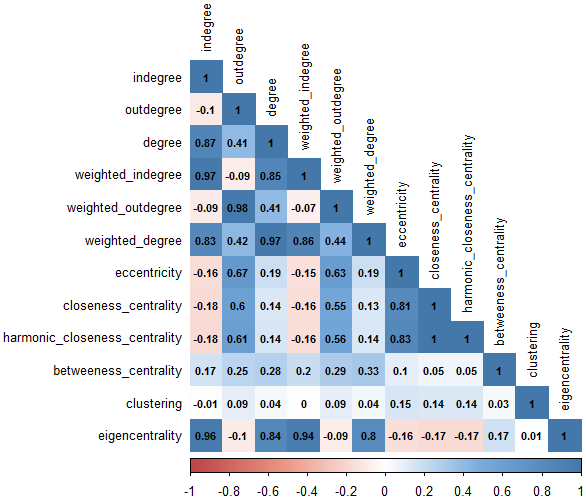
\includegraphics[width=.75\textwidth]{corr-matrix-brexit} %  % Correlation matrix
\end{figure}

\subsection{Graphs Visualization}
While mathematical metrics are essential to test hypotheses and draw sound conclusions, only a visual representation allows grasping the overall structure of a network quickly. Therefore, we show the five selected networks\footnote{Only interacting nodes are included.} in Figure \vref{network-graphs} to describe the collected data visually. These topic-network structures seem to differ on many network measures. Nevertheless, we can identify some shared features.
% Network graphs
\begin{figure}[t]
  \caption{Network graphs per topic.}\label{network-graphs}
  \begin{subfigure}[t]{.33\textwidth}
    \centering
    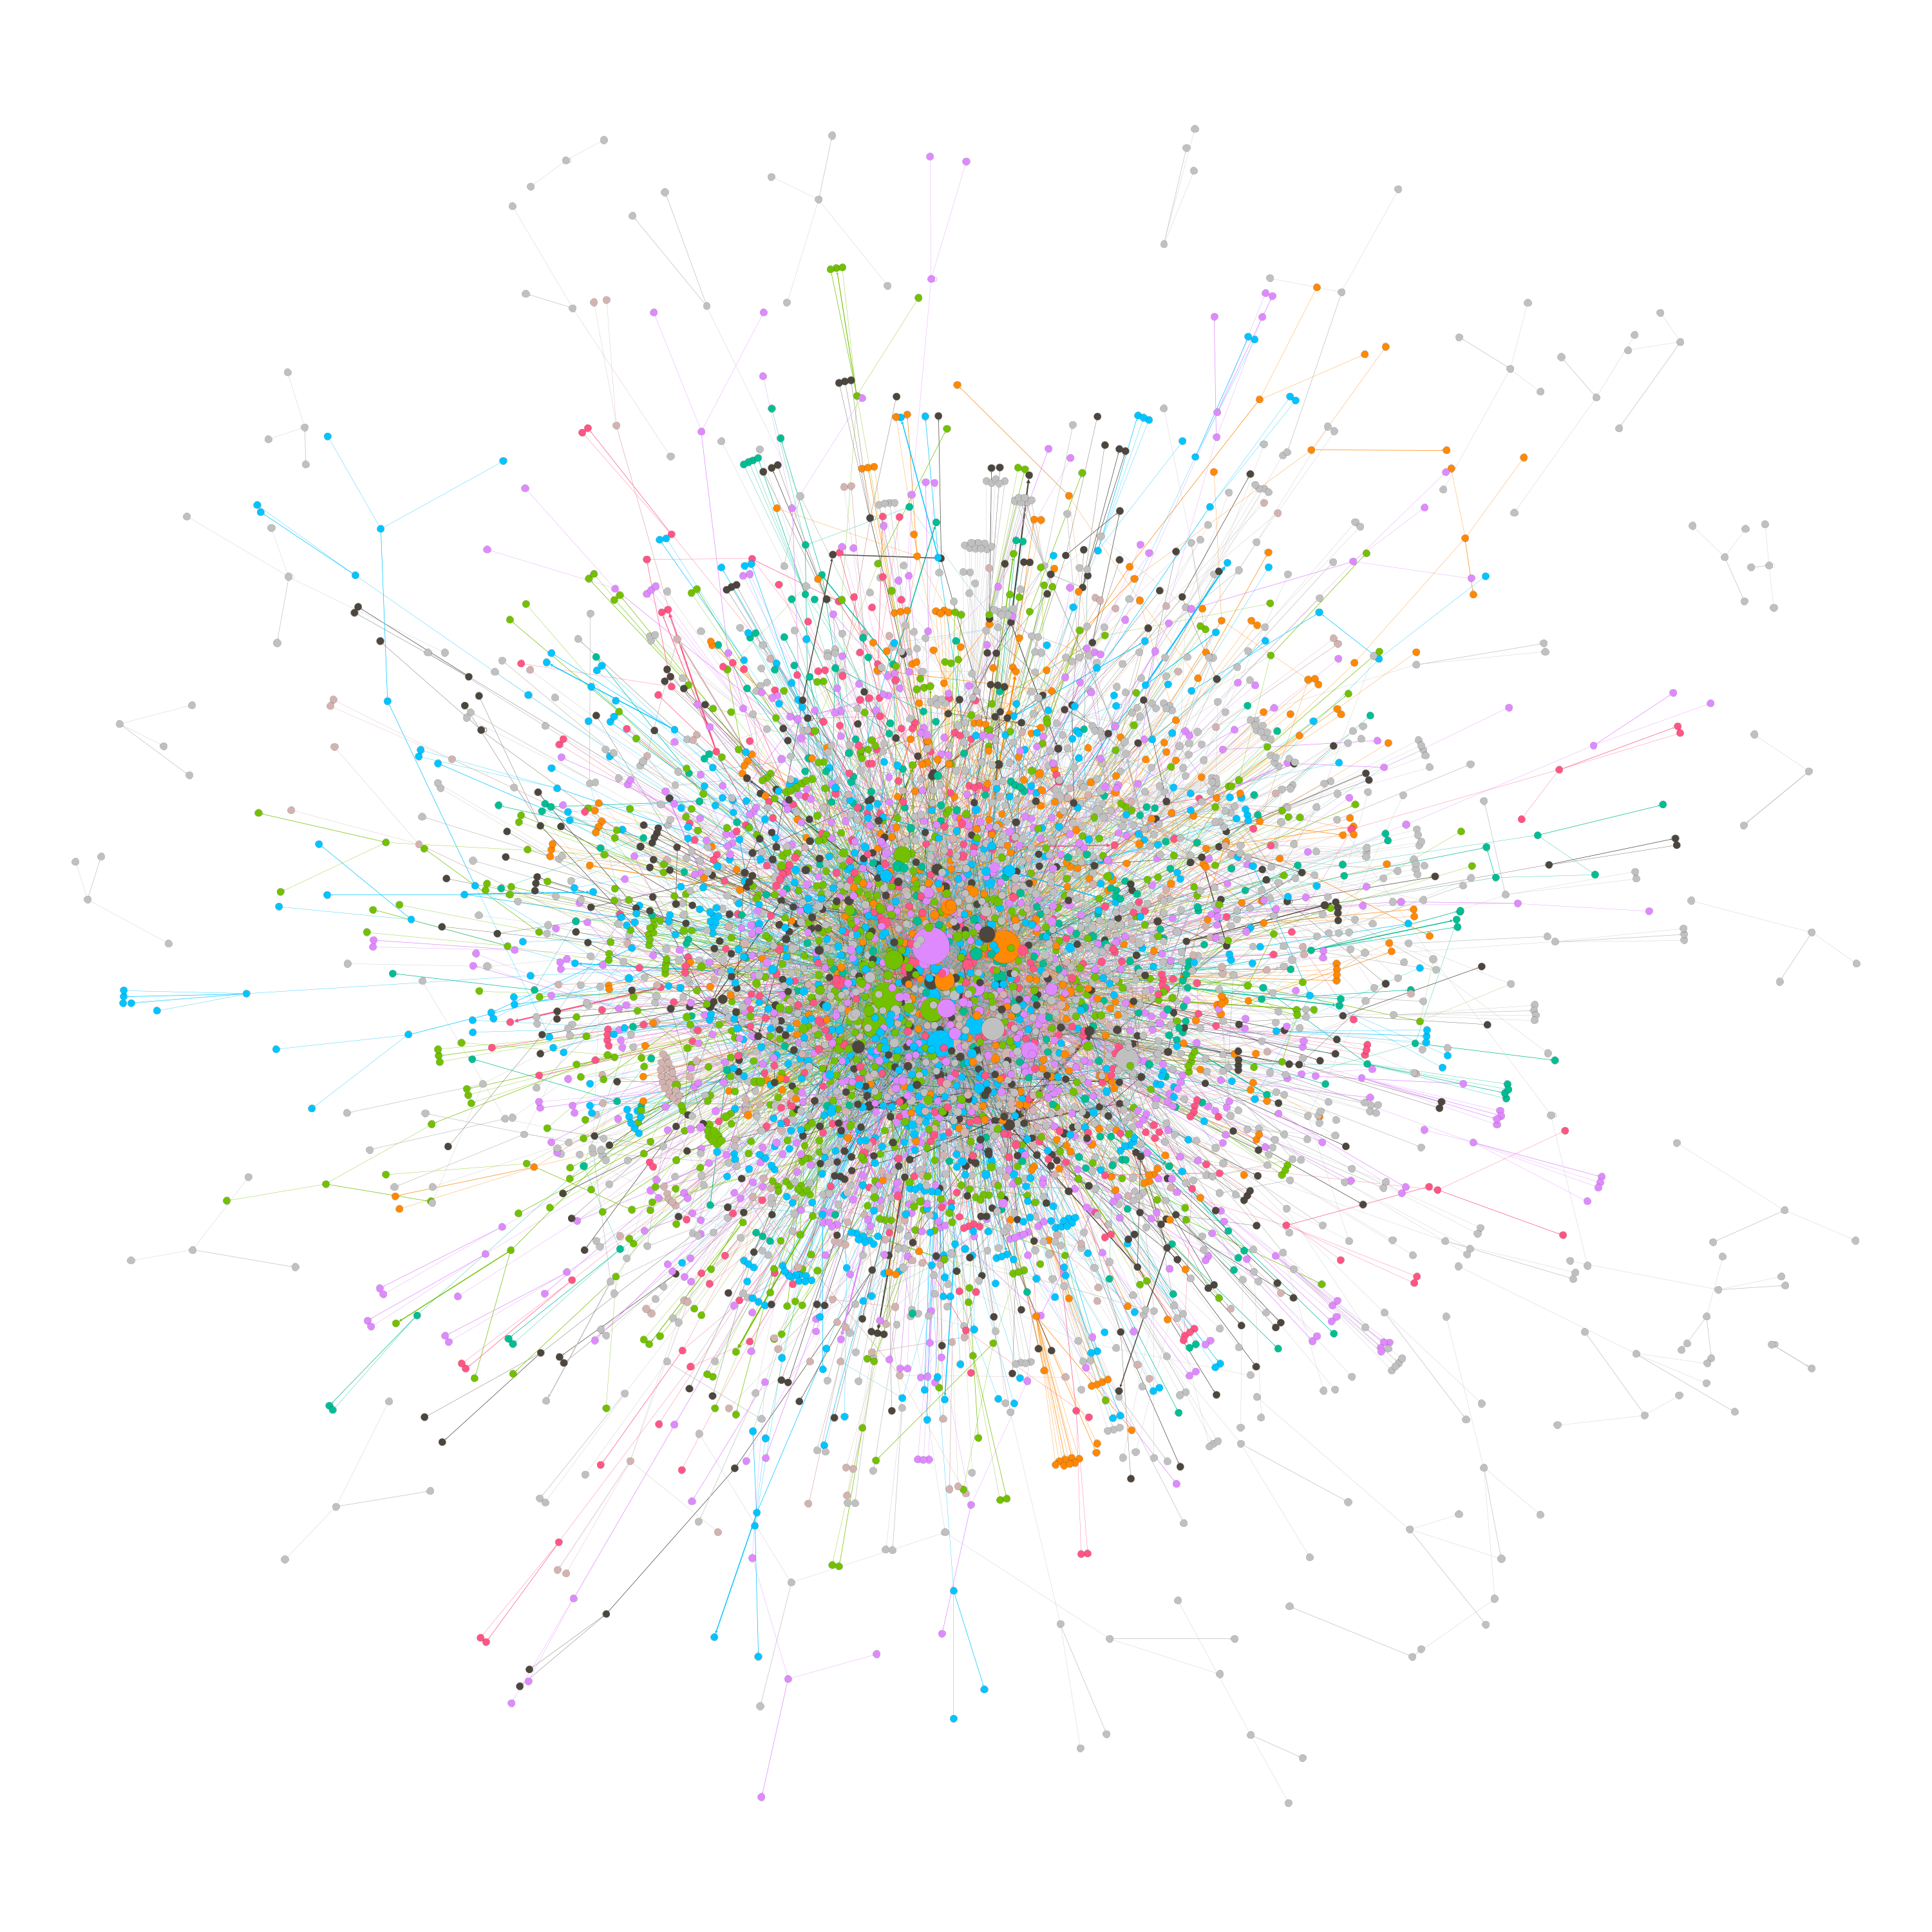
\includegraphics[width=1\linewidth]{brexit}
    \caption{Brexit}
  \end{subfigure}%
  \begin{subfigure}[t]{.33\textwidth}
    \centering
    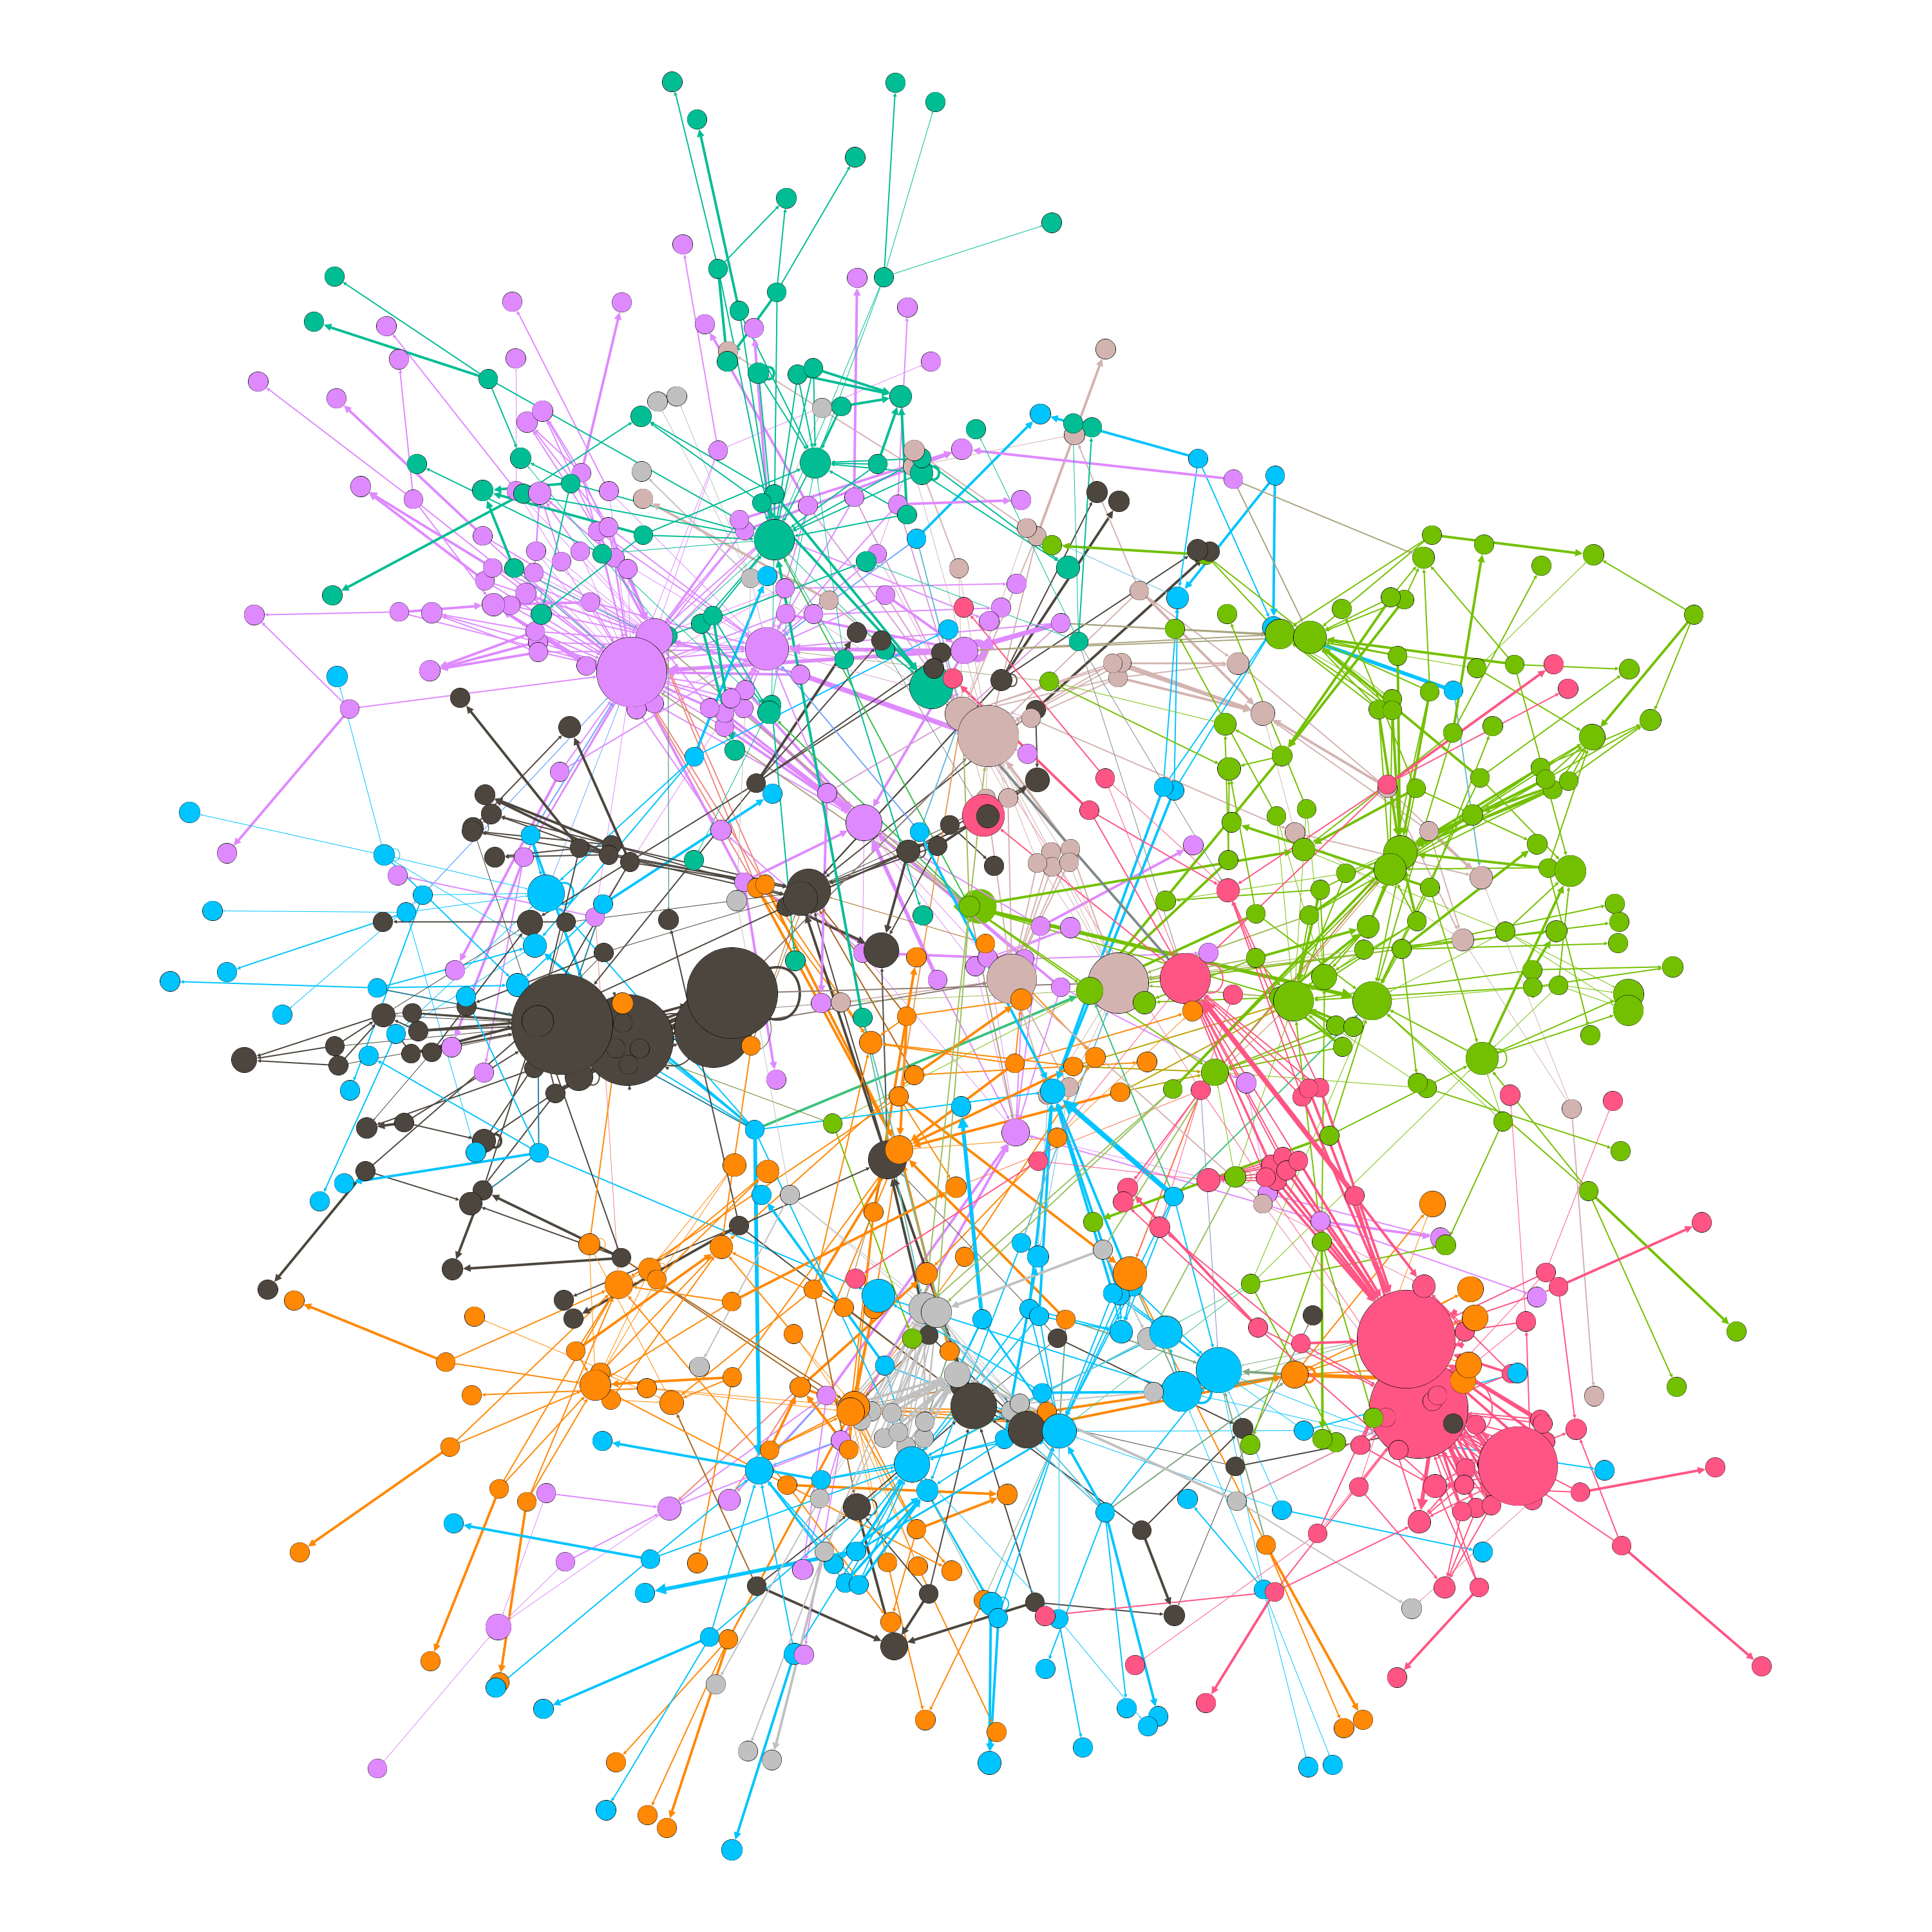
\includegraphics[width=1\linewidth]{populism}
    \caption{Populism}
  \end{subfigure}
  \begin{subfigure}[t]{.33\textwidth}
    \centering
    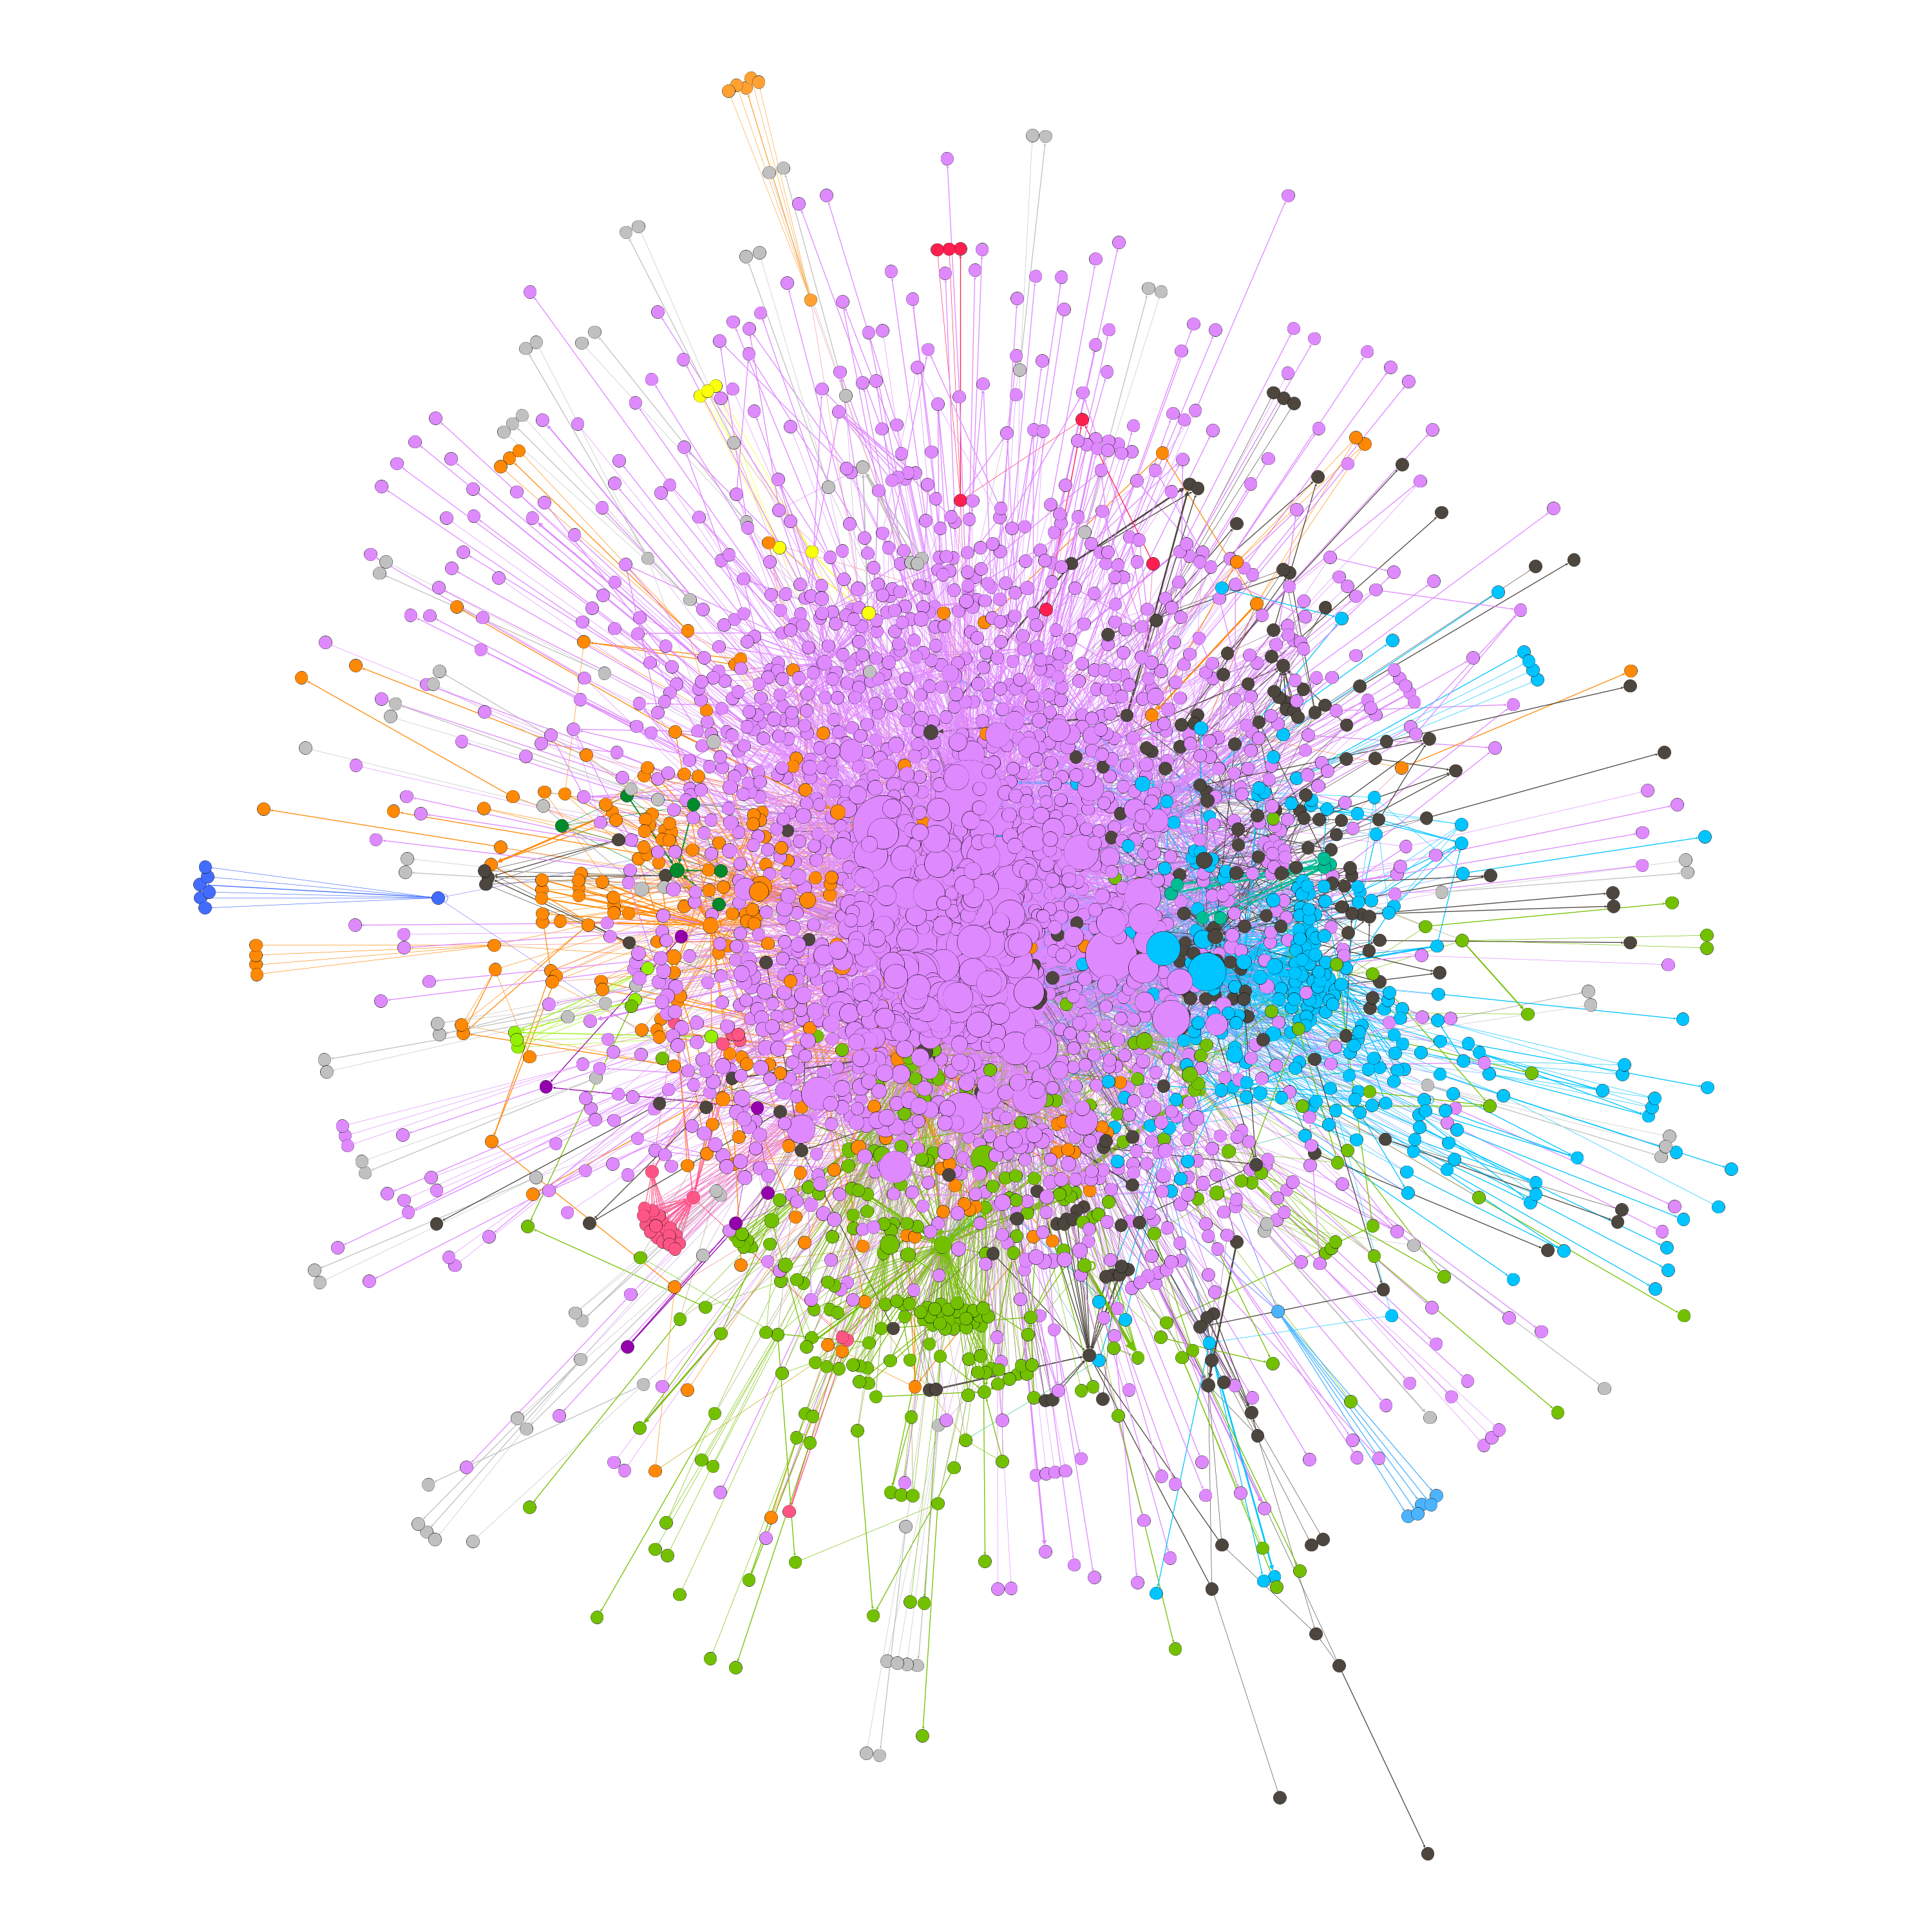
\includegraphics[width=1\linewidth]{refugees}
    \caption{Refugees}
  \end{subfigure}
  \newline
  \begin{subfigure}[t]{.5\textwidth}
    \centering
    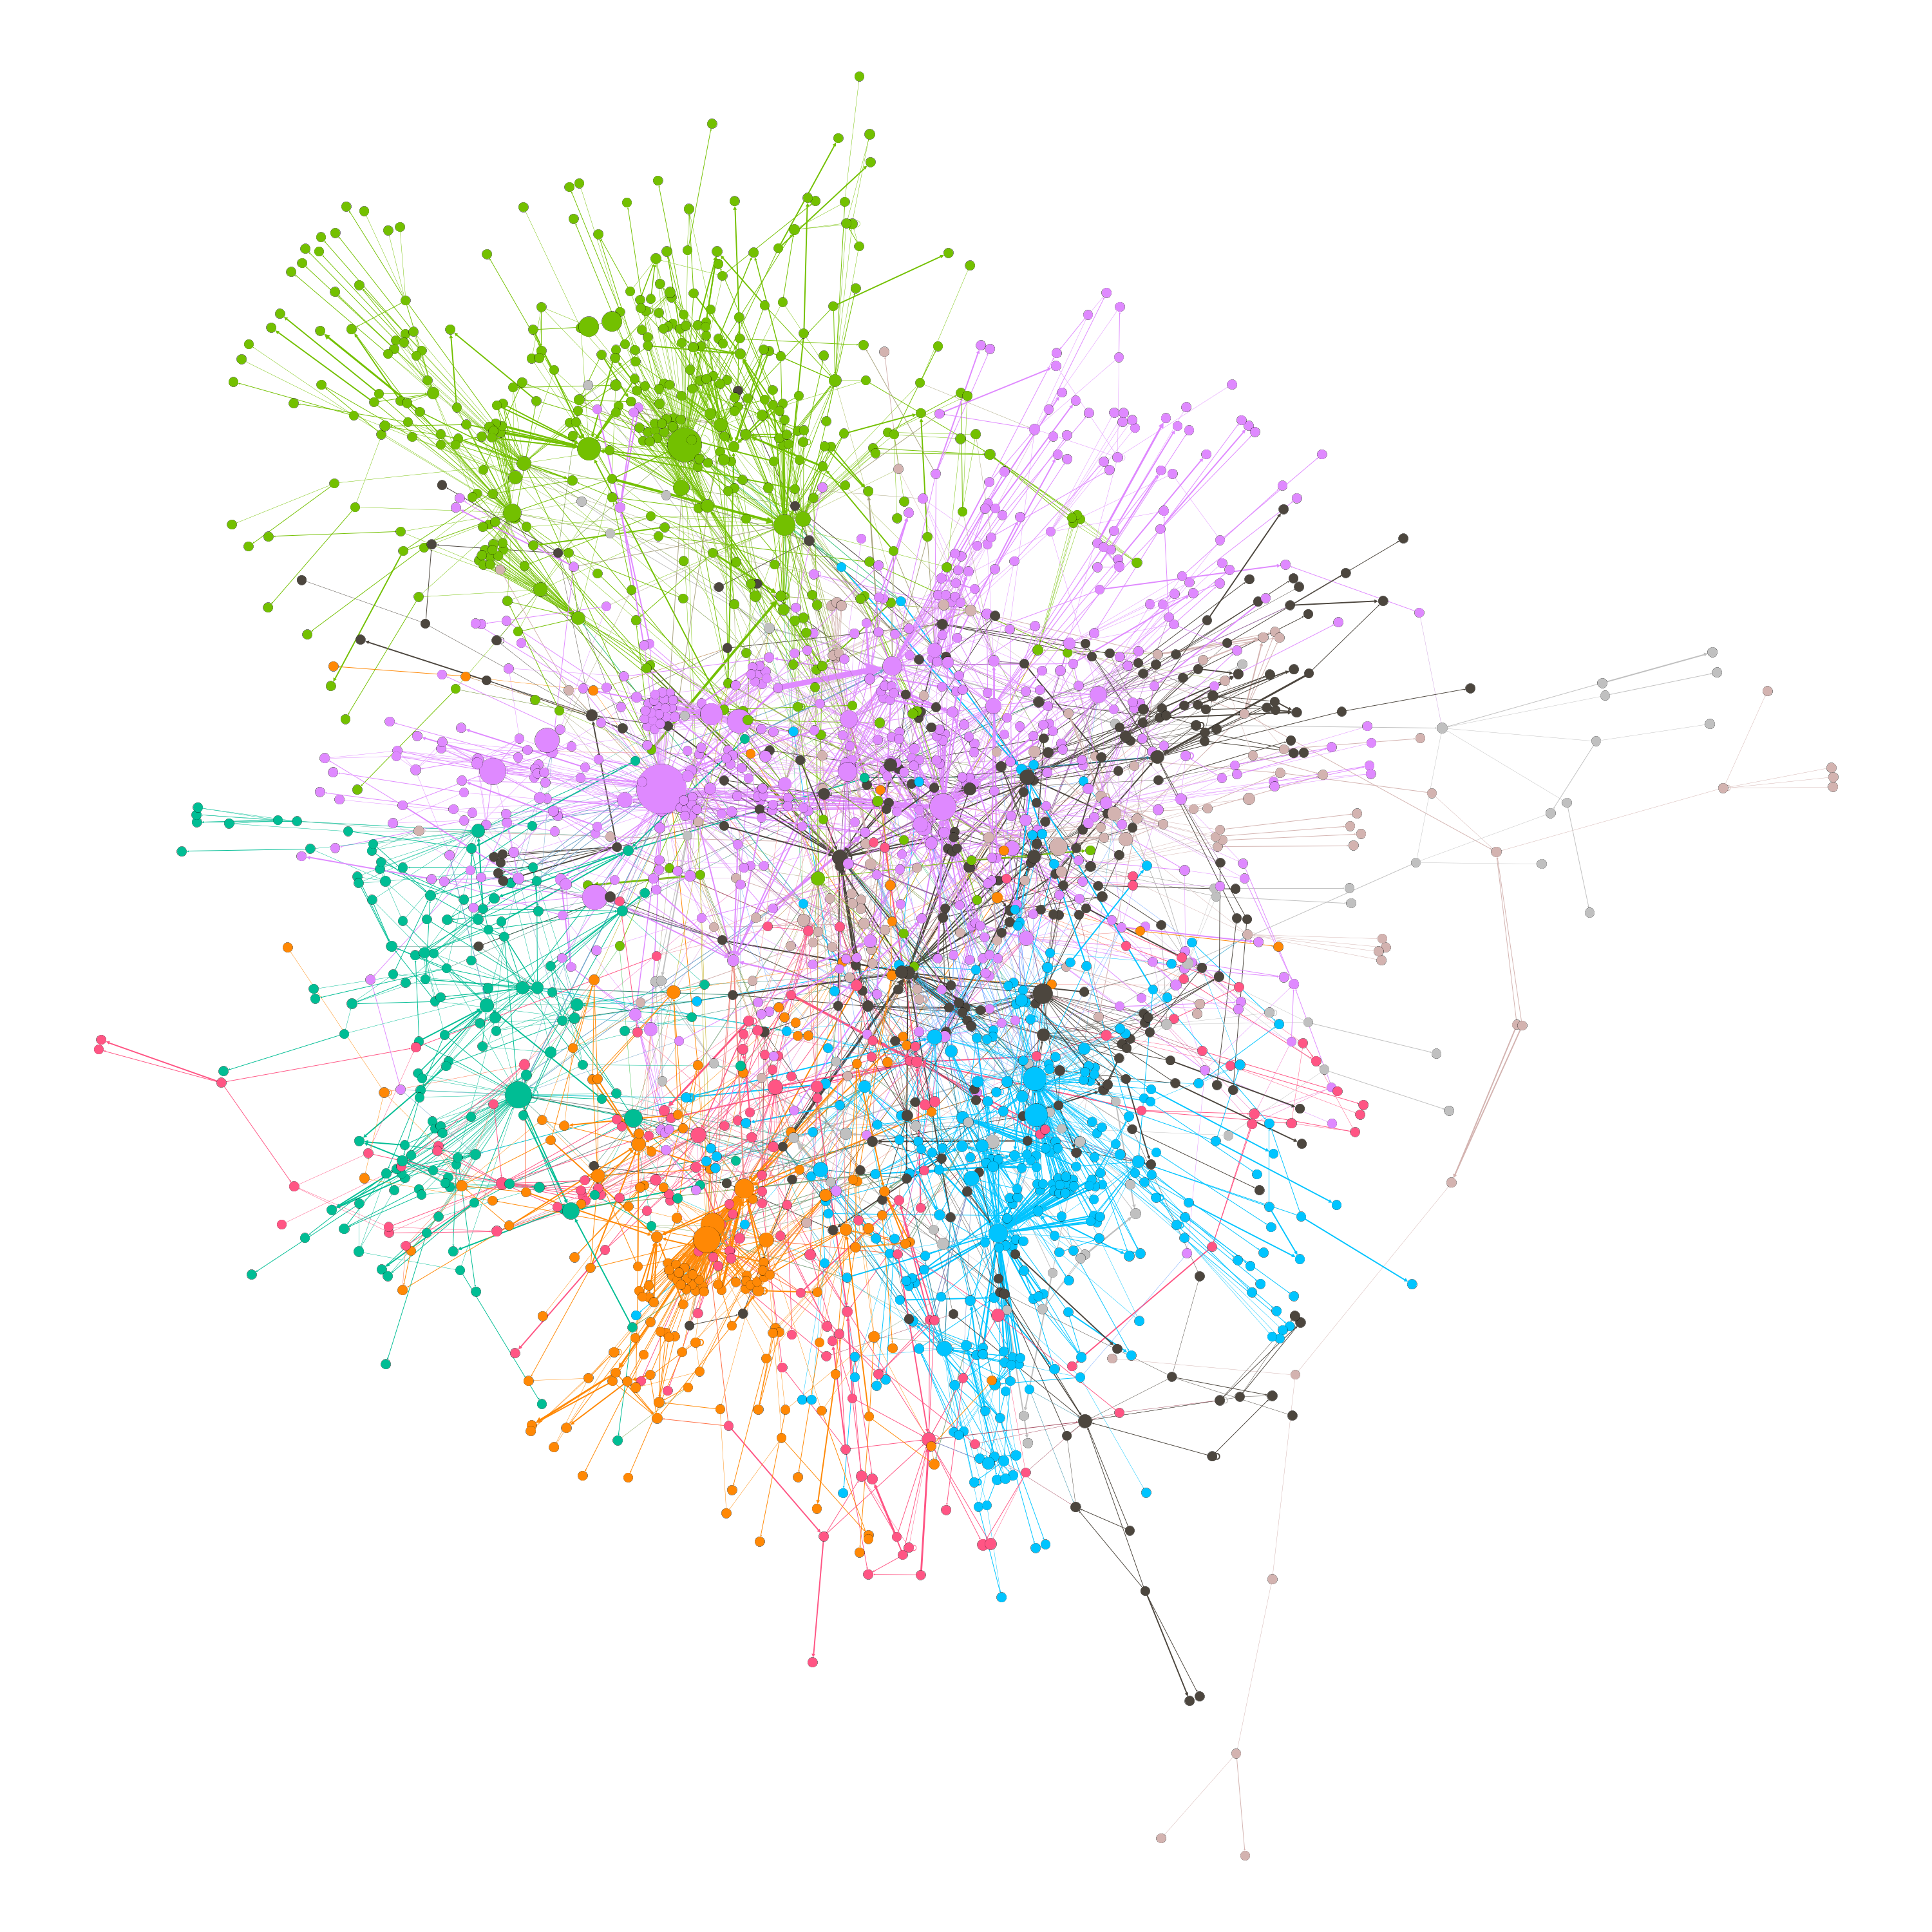
\includegraphics[width=.8\linewidth]{terrorism}
    \caption{Terrorism}
  \end{subfigure}%
  \begin{subfigure}[t]{.5\textwidth}
    \centering
    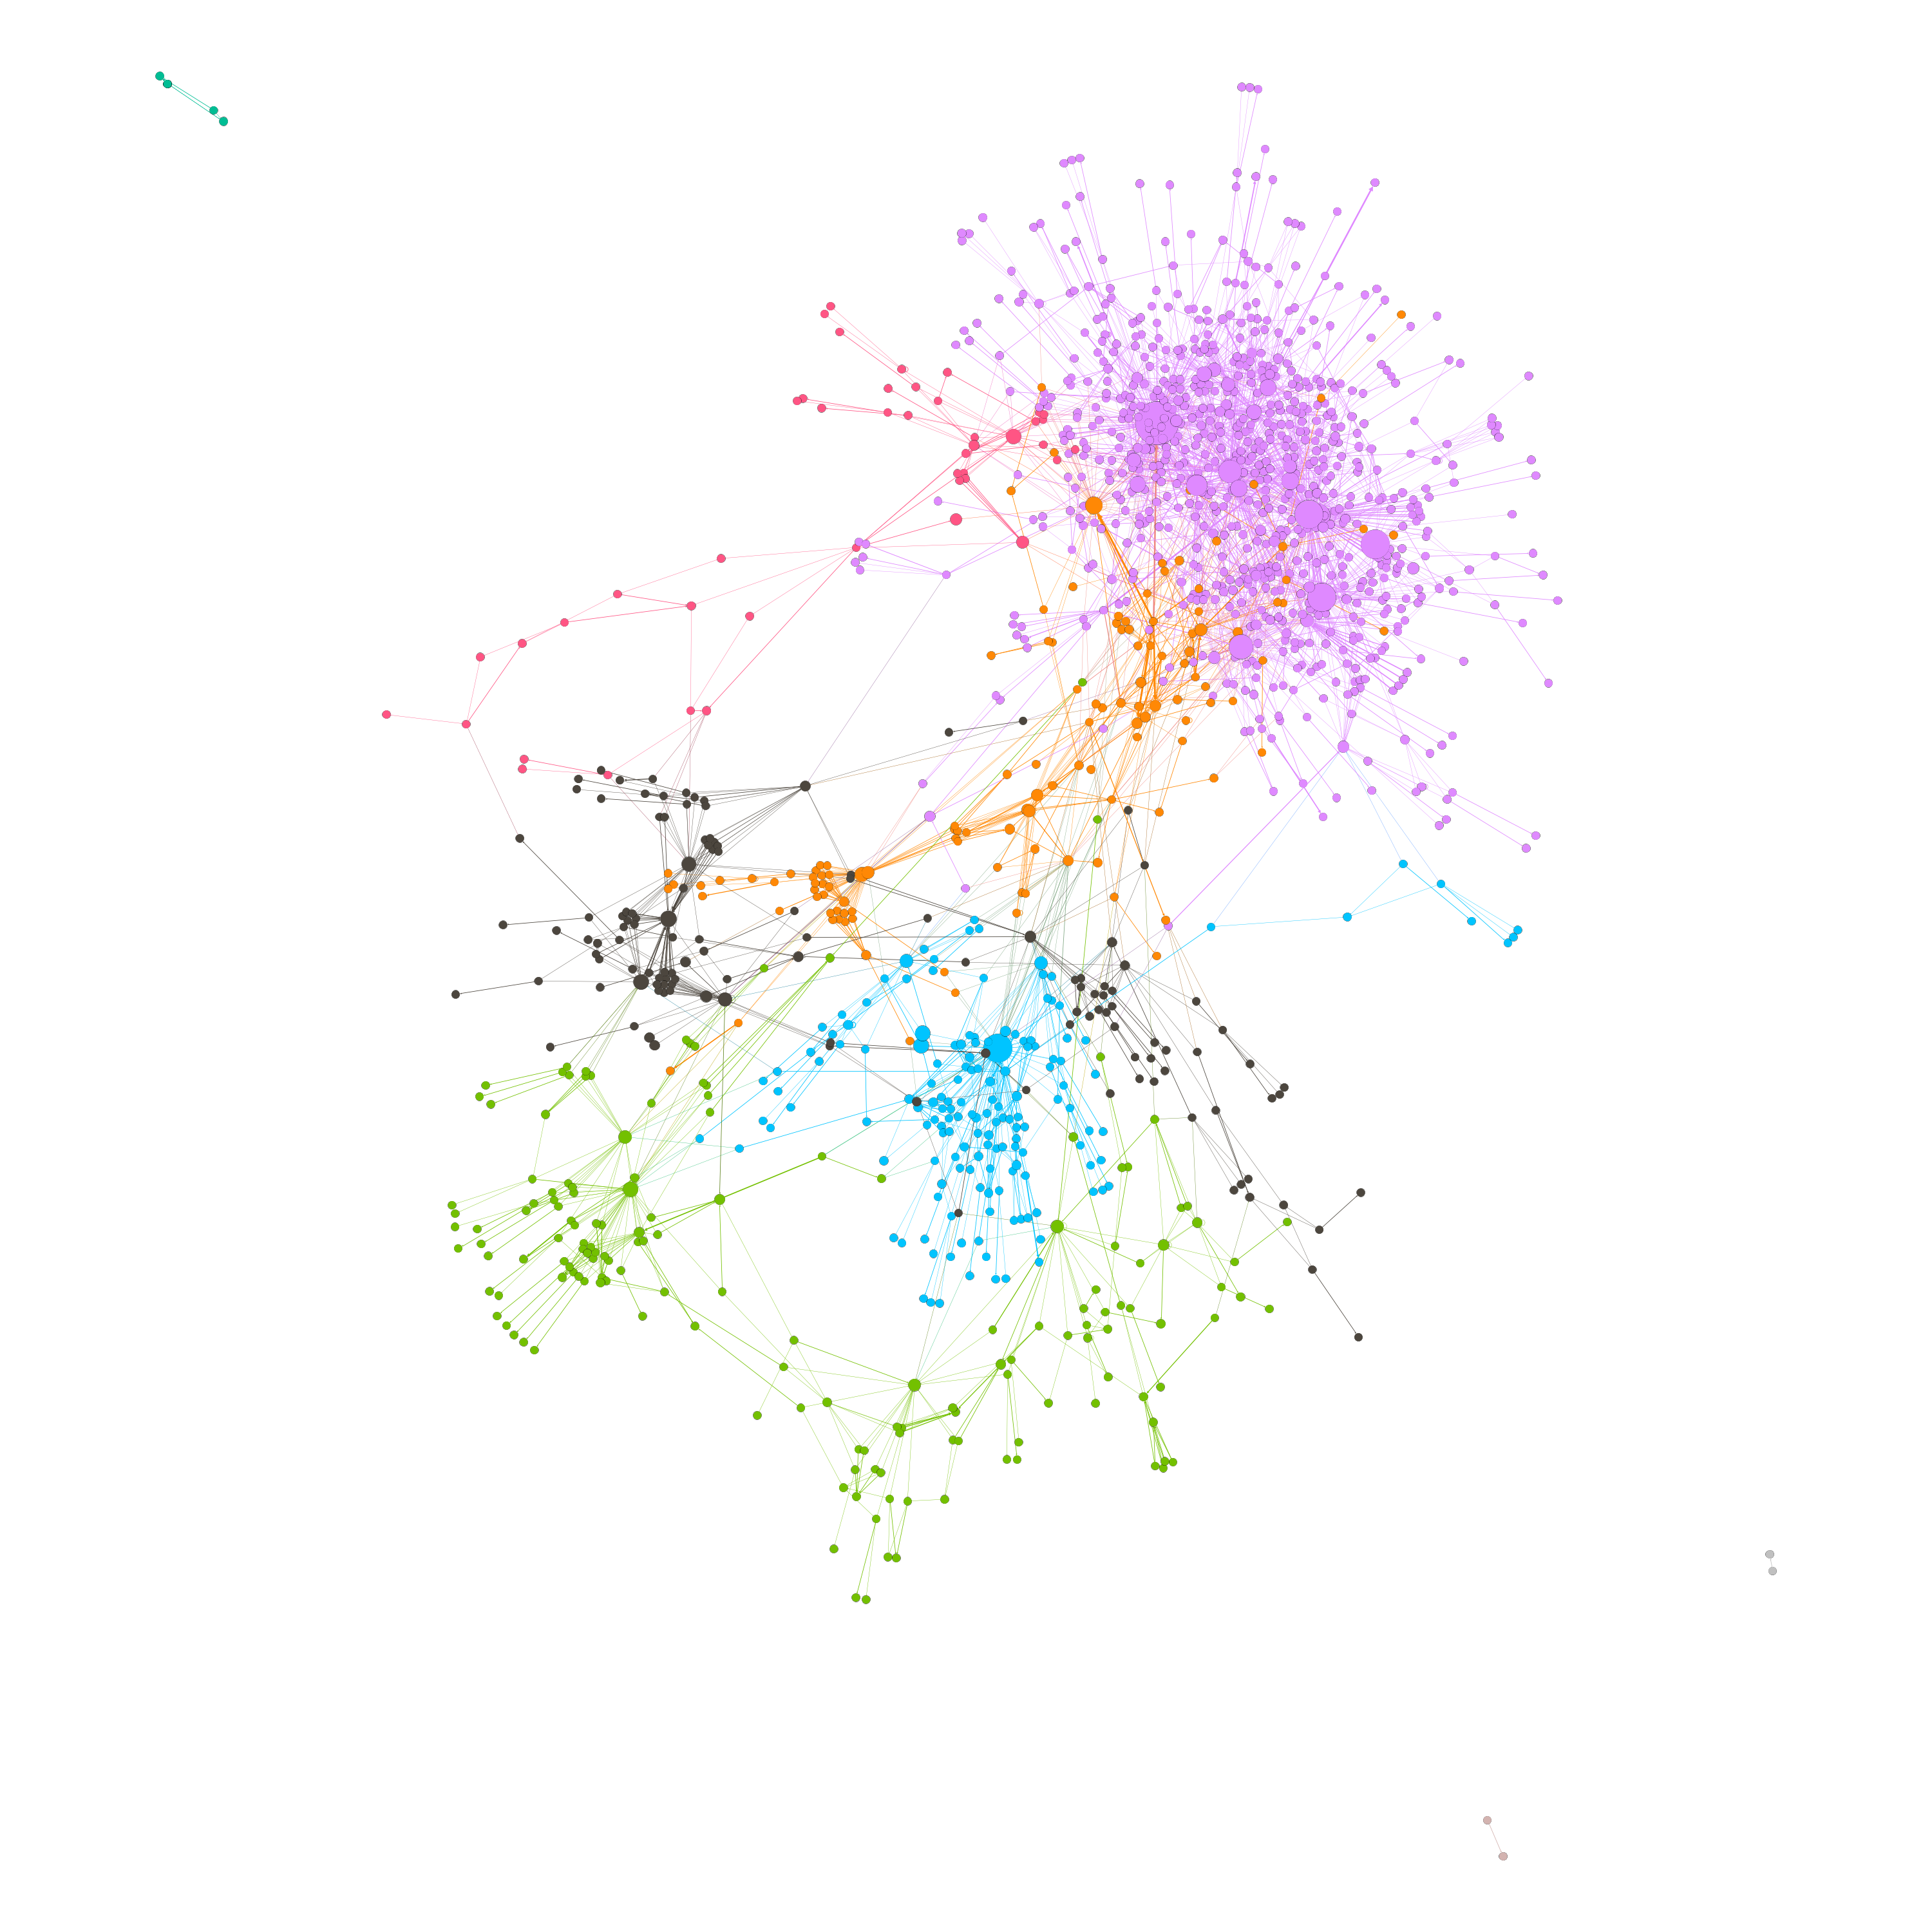
\includegraphics[width=.8\linewidth]{unemployment}
    \caption{Unemployment}
  \end{subfigure}
\end{figure}

The geographical position of nodes is determined by a force-vector algorithm\footnote{The Yifan Hu's algorithm, in our case, as mentioned earlier.} that simulates a system of physical forces: nodes tend to repulse each other, while edges hold back bounding nodes. The algorithm changes the disposition of nodes until it reaches an equilibrium where a balance of forces is guaranteed by minimizing the number of edges crossings. In other words, two nodes are closer if they are connected with each other or to the same set of nodes. Once the equilibrium is reached, the relative position of nodes reveals clusters and structural holes – the empty zone between clusters –  in the network. The color of nodes in our networks represents the community to which they belong to, determined by the modularity. Lastly, the size of the nodes represents their (eigenvector) centrality in the network.

We can classify our networks into two main groups. \texttt{Brexit} and \texttt{refugees} appear as a one, highly dense cluster, with almost no subclusters or structural holes and many sparse nodes around it. Few central individuals, called hubs, attract many connections in a star structure, where the surrounding nodes are connected to the center but not among them.

On the other hand, \texttt{populism} and \texttt{terrorism} show many small and dense subclusters, while \texttt{unemployment} has three distant and massive clusters.
